\documentclass[a4paper]{article}
\usepackage[utf8]{inputenc}
\usepackage[russian]{babel}
\usepackage[T2]{fontenc}
\usepackage[warn]{mathtext}
\usepackage{graphicx}
\usepackage{amsmath}
\usepackage{floatflt}
\usepackage{tikz}
\usepackage{pgfplots}
\usepackage[left=20mm, top=20mm, right=20mm, bottom=20mm, footskip=10mm]{geometry}


\graphicspath{ {images/} }
\usepackage{multicol}
\setlength{\columnsep}{2cm}


\begin{document}

\begin{titlepage}
	\centering
	\vspace{5cm}
	\vspace{4cm}
	{\scshape\Large Лабораторная работа 3.2.3\par}
	\vspace{1cm}
	{\huge\bfseries Резонанс токов в параллельном контуре\par}
	\vspace{1cm}
	\vfill
\begin{flushright}
	\vspace{0.3cm}
	{\LARGE Выполнил: Тимонин Андрей}
\end{flushright}
	

	\vfill

% Bottom of the page
	Долгопрудный, 2023 г.
\end{titlepage}

\section{Цель работы}

Исследование резонанса токов в параллельном колебательном контуре с изменяемой ёмкостью, включающее получение амплитудно-частотных и фазово-частотных характеристик, а также определение основных параметров контура.

\section{В работе используются:}
\begin{itemize}
    \item генератор сигналов
    \item источник напряжения, нагруженный на параллельный колебательный контур с переменной ёмкостью
    \item двухканальный осциллограф
    \item цифровые вольтметры
\end{itemize}


\section{Cхема установки}

Схема экспериментального стенда для изучения резонанса токов в параллельном колебательном контуре показана на рис. 1. Синусоидальный сигнал от генератора GFG-8255A поступает на вход источника тока. Представлен резистор, переменное напряжение, на котором в используемой схеме равно напряжению на входе «+» операционного усилителя. \\

\begin{figure}[h]
    \centering
    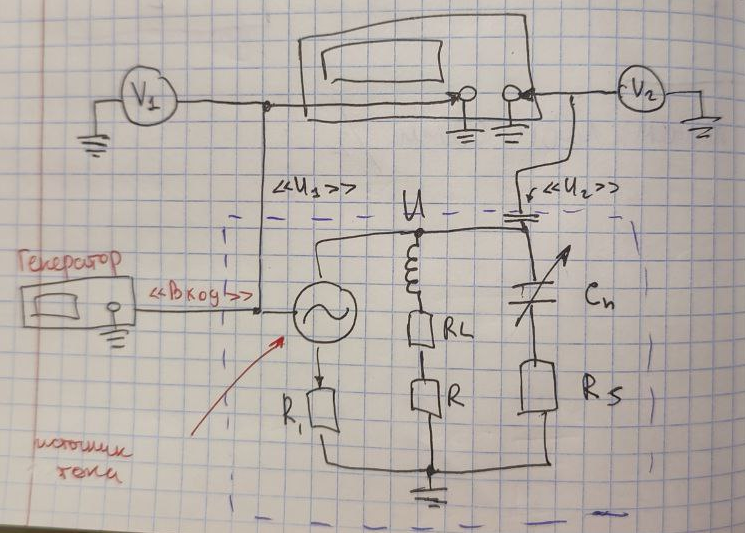
\includegraphics[width=10cm]{exper_setup.png}
    \caption{Схема экспериментального стенда}
    \label{fig:vac}
\end{figure}

Напряжение $ E = E_0cos(\omega t + \phi_0) $ поступает на вход «+» операционного усилителя от генератора через согласующую RC-цепочку. Это же напряжение через разъём «U1» подаётся одновременно на канал 1 осциллографа GOS-620 и вход 1-го цифрового вольтметра GDM-8245. Переменное напряжение на резисторе R1, как отмечалось выше, при этом также равно Е. Напряжение на контуре U, совпадающее с напряжением на конденсаторе, подаётся со знаком «–» через разъём «U2» на канал 2 осциллографа и вход 2-го цифрового вольтметра GDM-8245. Показанные на схеме установки ещё два конденсатора без наименований (помимо входящего в RC-цепочку) играют вспомогательную роль и не влияют на характеристики контура. Символ «->+» отмечает наличие источника питания полевого транзистора. Ток затвора «з» полевого транзистора ничтожно мал, так что токи истока «и» и стока «с» практически совпадают и равны току во внешней цепи контура. Как видно из схемы, \[ I = \frac{E}{R_1} = I_0cos(\omega t + \phi_0), \:\:\: I_0 = \frac{E_0}{R_1} \]


\section{Ход работы}

\begin{equation}\label{}
L=\frac{1}{C(2\pi f)^2} \\
\end{equation}
\begin{equation}\label{}
\rho=\frac{1}{2\pi fC} \\
\end{equation}
\begin{equation}\label{}
Z_{\text{рез}}=\frac{U}{E_0}R_1
\end{equation}
\begin{equation}\label{}
Q=\frac{UR_1}{E_0}2\pi fC
\end{equation}
\begin{equation}\label{}
R_{\sum}=\frac{E_0}{UR_1}\frac{1}{(2\pi fC)^2}
\end{equation}
\begin{equation}\label{}
R_{Smax}=10^{-3}\cdot\frac{1}{\omega_0C}
\end{equation}
\begin{equation}\label{}
R_L=\frac{E_0}{UR_1}\frac{1}{(2\pi fC)^2}-R-10^{-3}\cdot\frac{1}{\omega_0C}
\end{equation}

    \begin{table}[b!]
	\centering
	\caption{Результаты расчетов для пункта 11}
\begin{tabular}{|c|c|c|c|c|c|}
	\hline
	$ C_n, \text{нФ} $ & $ f_{0n} $, кГц & $ U_{0n}, $ B & $ E $, B & $ L $, мкГн & $ \rho $, Ом \\
	\hline
25.1 & $32.13\pm 0.01$&  $1.1927\pm 0.0001$&  $0.2062\pm 0.0001$&  $978.434\pm 49.531$&  $197.437 \pm 9.933$ \\ \hline
33.2 &  $27.81\pm 0.01$&  $0.7473\pm 0.0001$&  $0.2060\pm 0.0001$&  $987.579\pm 50.089$&  $172.471\pm 8.686$\\ \hline
47.3 & $23.13\pm 0.01$ &  $0.6656\pm 0.0001$&  $0.2062\pm 0.0001$&  $1002.435\pm 50.989$&  $145.579\pm 7.342$ \\ \hline
57.4 &  $21.23\pm 0.01$&  $0.5729\pm 0.0001$&  $0.2062\pm 0.0001$&  $979.727\pm 49.909$& $130.646\pm 6.594$ \\ \hline
67.5 &  $19.56\pm 0.01$&  $0.4503\pm 0.0001$&  $0.2060\pm 0.0001$& $981.435\pm 50.075$&  $120.581 \pm 6.091$\\ \hline 
82.7 & $17.70\pm 0.01$ &  $0.3886\pm 0.0001$&  $0.2060\pm 0.0001$& $978.653\pm 50.038$ & $108.783\pm 5.501$ \\ \hline 
101.6 &  $15.99\pm 0.01$ &  $0.3364\pm 0.0001$&  $0.2059\pm 0.0001$&  $976.457\pm 50.044$&  $98.035\pm 4.963$\\ \hline
\end{tabular}

\end{table}% 

    \begin{table}
	\centering
	\caption{Результаты расчетов для пункта 11}
\begin{tabular}{|c|c|c|c|c|}
	\hline
	$ Z_{\text{рез}} $, Ом & $ Q $ & $ R_\Sigma,  $ Ом & $ R_{Sm} $, Ом & $ R_L $, Ом \\
	\hline
$5830.464\pm 586.363$& $29.531\pm 4.456$& $6.686\pm 1.345$& $0.197\pm 0.010$& $2.988\pm 1.705$ \\ \hline
$3656.691\pm 367.934$& $21.202\pm 3.201$& $8.135\pm 1.638$& $0.172\pm 0.009$& $4.462\pm 1.997$\\ \hline
$3253.758\pm 327.443$& $22.351\pm 3.376$& $6.513\pm 1.312$& $0.146\pm 0.007$& $2.868\pm 1.670$\\ \hline
$2800.597\pm 281.907$& $21.437\pm 3.240$& $6.095\pm 1.229$& $0.131\pm 0.007$& $2.464\pm 1.585$\\ \hline
$2203.410\pm 221.900$& $18.273\pm 2.763$& $6.599\pm 1.331$& $0.121\pm 0.006$& $2.978\pm 1.687$\\ \hline
$1901.499\pm 191.562$& $17.480\pm 2.645$& $6.223\pm 1.256$& $0.109\pm 0.006$& $2.615\pm 1.612$\\ \hline
$1646.873\pm 165.977$& $16.799\pm 2.543$& $5.836\pm 1.179$& $0.098\pm 0.005$& $2.238\pm 1.534$\\ \hline

\end{tabular}

\end{table}% 
\vspace{5}
    \begin{table}[b!]
	\centering
	\caption{Результаты расчетов для пункта 11}
\begin{tabular}{|c|c|c|c|}
\hline
$L_{sred}$& 983.531& $RL_{sred}$& 2.945\\ \hline
$\triangle L_{sred}$& 50.097 & $\triangle RL_{sred}$& 1.684\\ \hline
$S_{L_{\text{сред}}}$& 3.077& $S_{RL_{\text{сред}}}$& 0.226\\ \hline
$\triangle_{\text{случ}}L_{sred}$ & 7.530& $\triangle_{\text{случ}}RL_{sred}$& 0.553\\ \hline


\end{tabular}

\end{table}% 
    \begin{table}
        \centering
        \begin{tabular}{|c|c|c|}
            \cline{1-3}
            №  & $f_{0n}$, \text{кГц} & U, \text{В} \\ \cline{1-3}
            1  & $18.79\pm 0.01$ & $0.2680\pm 0.0001$  \\ \cline{1-3}
            2  & $20.10\pm 0.01$  & $0.2940\pm 0.0001$ \\ \cline{1-3}
            3  & $20.20\pm 0.01$  & $0.2760\pm 0.0001$  \\ \cline{1-3}
            4  & $18.90\pm 0.01$  & $0.3100\pm 0.0001$   \\ \cline{1-3} 
            5  & $19.26\pm 0.01$ & $0.4300\pm 0.0001$   \\ \cline{1-3} 
            6  & $19.05\pm 0.01$ & $0.3500\pm 0.0001$   \\ \cline{1-3}
            7  & $18.95\pm 0.01$ & $0.3100\pm 0.0001$   \\ \cline{1-3}
            8  & $18.96\pm 0.01$ & $0.3200\pm 0.0001$   \\ \cline{1-3} 
            9  & $19.45\pm 0.01$ & $0.4650\pm 0.0001$ \\ \cline{1-3}
            10 & $19.33\pm 0.01$ & $0.4440\pm 0.0001$ \\ \cline{1-3} 
            11 & $19.26\pm 0.01$ & $0.4240\pm 0.0001$  \\ \cline{1-3}
            12 & $19.23\pm 0.01$ & $0.4180\pm 0.0001$ \\ \cline{1-3}
            13 & $19.15\pm 0.01$ & $0,3900\pm 0.0001$   \\ \cline{1-3}
            14 & $18.90\pm 0.01$  & $0.3000\pm 0.0001$    \\ \cline{1-3}
            15 & $19.10\pm 0.01$  & $0.3700\pm 0.0001$   \\ \cline{1-3}
            16 & $19.79\pm 0.01$ & $0.4000\pm 0.0001$    \\ \cline{1-3}
            17 & $19.70\pm 0.01$ & $0.4200\pm 0.0001$   \\ \cline{1-3}
            18 & $19.97\pm 0.01$ & $0.3400\pm 0.0001$   \\ \cline{1-3}
            19 & $19.98\pm 0.01$ & $0.3370\pm 0.0001$  \\ \cline{1-3}
            20 & $20.40\pm 0.01$  & $0.2300\pm 0.0001$   \\ \cline{1-3}
        \end{tabular}
        \caption{Данные для пункта 9 при n = 3}
        \label{tab:my_label}
    \end{table}

    \begin{tikzpicture}[b]
    \begin{axis}
    [
        xlabel={$f_{0n}$, \text{кГц}}, 
        ylabel={$U, \text{В}$}, 
        grid,
        height = 0.4\paperheight, 
	width = 0.8\paperwidth,
        title={AЧХ при n = 3 и n = 5},
    ]
    
    \addplot[red, mark=x, only marks] plot [error bars/.cd, y dir = both, y explicit]
    table[x =x, y =y, y error =ey, x error =ex]{U_f_1.txt};
    \addplot[blue, mark=x, only marks] plot [error bars/.cd, y dir = both, y explicit]
    table[x =x, y =y, y error =ey, x error =ex]{U_f_2.txt};
    \addlegendentry{n = 3}
    \addlegendentry{n = 5}
    
    \end{axis}
    \end{tikzpicture}
    

    \begin{tikzpicture}
    \begin{axis}
    [
        xlabel={$f_{0n}$, \text{кГц}}, 
        ylabel={$U, \text{В}$}, 
        grid,
        height = 0.4\paperheight, 
	width = 0.8\paperwidth,
        title={AЧХ при n = 3},
    ]
    
    \addplot[red, mark=x, only marks] plot [error bars/.cd, y dir = both, y explicit]
    table[x =x, y =y, y error =ey, x error =ex]{U_f_1.txt};
    \addlegendentry{n = 3}
    
    \end{axis}
    \end{tikzpicture}
    

    \begin{tikzpicture}
    \begin{axis}
    [
        xlabel={$f_{0n}$, \text{кГц}}, 
        ylabel={$U, \text{В}$}, 
        grid,
        legend pos=north west,
        height = 0.4\paperheight, 
	width = 0.8\paperwidth,
        title={AЧХ при n = 5},
    ]
    
    \addplot[blue, mark=x, only marks] plot [error bars/.cd, y dir = both, y explicit]
    table[x =x, y =y, y error =ey, x error =ex]{U_f_2.txt};

    \addlegendentry{n = 5}
    
    \end{axis}
    \end{tikzpicture}

    \begin{table}
        \centering
        \begin{tabular}{|c|c|c|}
            \cline{1-3}
            №  & $f_{0n}$, \text{кГц} & U, \text{В} \\ \cline{1-3}
            1  & $22.65\pm 0.01$  & $0.4400\pm 0.0001$   \\ \cline{1-3}
            2  & $22.55\pm 0.01$  & $0.3900\pm 0.0001$   \\ \cline{1-3}
            3  & $22.57\pm 0.01$  & $0.4050\pm 0.0001$  \\ \cline{1-3}
            4  & $23.86\pm 0.01$ & $0.4150\pm 0.0001$ \\ \cline{1-3} 
            5  & $23.46\pm 0.01$  & $0.5950\pm 0.0001$  \\ \cline{1-3}
            6  & $22.85\pm 0.01$  & $0.5350\pm 0.0001$  \\ \cline{1-3}
            7  & $23.24\pm 0.01$  & $0.6660\pm 0.0001$ \\ \cline{1-3}
            8  & $23.78\pm 0.01$  & $0.4440\pm 0.0001$  \\ \cline{1-3}
            9  & $23.91\pm 0.01$  & $0.3900\pm 0.0001$   \\ \cline{1-3}
            10 & $23.37\pm 0.01$  & $0.6350\pm 0.0001$  \\ \cline{1-3}
            11 & $23.65\pm 0.01$  & $0.9100\pm 0.0001$   \\ \cline{1-3}
            12 & $23.78\pm 0.01$  & $0.4440\pm 0.0001$  \\ \cline{1-3}
            13 & $22.60\pm 0.01$  & $0.4170\pm 0.0001$  \\ \cline{1-3}
            14 & $22.62\pm 0.01$  & $0.4260\pm 0.0001$  \\ \cline{1-3}
            15 & $22.13\pm 0.01$  & $0.2740\pm 0.0001$  \\ \cline{1-3}
            16 & $23.85\pm 0.01$  & $0.4140\pm 0.0001$  \\ \cline{1-3}
        \end{tabular}
        \caption{Данные для пункта 9 при n = 5}
        \label{tab:my_label}
    \end{table}

    \begin{table}
    \centering
        \begin{tabular}{|c|c|c|c|c|}
        \cline{1-5}
        №  & $f_{0n}$, \text{кГц} & x & $\triangle x$ & $\triangle \varphi$ \\ \cline{1-5}
        1 & $21.42\pm 0.01$ & $8.0\pm 0.5$   & $5.0\pm 1.0$   & $\frac{8}{13}$     \\ \cline{1-5} 
        2 & $21.88\pm 0.01$ & $6.0\pm 0.5$  & $4.5\pm 1.0$ & $\frac{6}{10.5}$   \\ \cline{1-5}
        3 & $21.95\pm 0.01$ & $6.0\pm 0.5$   & $4.5\pm 1.0$ & $\frac{6}{10.5}$   \\ \cline{1-5}
        4 & $22.12\pm 0.01$ & $6.5\pm 0.5$ & $4.0\pm 1.0$   & $\frac{6.5}{10.5}$ \\ \cline{1-5}
        5 & $22.37\pm 0.01$ & $7.0\pm 0.5$   & $4.0\pm 1.0$  & $\frac{7}{11}$     \\ \cline{1-5}
        6 & $22.54\pm 0.01$ & $7.0\pm 0.5$   & $3.5\pm 1.0$ & $\frac{7}{10.5}$   \\ \cline{1-5}
        7 & $22.70\pm 0.01$  & $7.2\pm 0.5$ & $3.0\pm 1.0$   & $\frac{7.2}{10.2}$ \\ \cline{1-5}
        8 & $22.83\pm 0.01$ & $8.0\pm 0.5$   & $2.8\pm 1.0$ & $\frac{8}{10.8}$   \\ \cline{1-5}
        9 & $22.94\pm 0.01$ & $16.0\pm 0.5$  & $4.0\pm 1.0$   & $\frac{16}{20}$    \\ \cline{1-5}
        10 & $23.33\pm 0.01$ & $21.0\pm 0.5$  & $1.0\pm 1.0$   & $\frac{21}{22}$    \\ \cline{1-5}
        11 & $23.53\pm 0.01$ & $23.0\pm 0.5$  & $3.5\pm 1.0$ & $\frac{23}{26.5}$  \\ \cline{1-5}
        12 & $23.80\pm 0.01$  & $24.0\pm 0.5$ & $5.0\pm 1.0$   & $\frac{24}{29}$    \\ \cline{1-5}
        13 & $24.00\pm 0.01$    & $25.0\pm 0.5$  & $6.0\pm 1.0$   & $\frac{25}{31}$    \\ \cline{1-5}
        14 & $24.28\pm 0.01$ & $26.0\pm 0.5$  & $7.0\pm 1.0$   & $\frac{26}{33}$    \\ \cline{1-5}
        15 & $25.00\pm 0.01$    & $26.0\pm 0.5$  & $8.0\pm 1.0$   & $\frac{26}{34}$    \\ \cline{1-5}
        16 & $24.70\pm 0.01$  & $26.0\pm 0.5$  & $8.0\pm 1.0$   & $\frac{26}{34}$   \\ \cline{1-5}
        \end{tabular}
        \caption{Данные для пункта 10 при n = 3}
        \label{tab:my_label}
    \end{table}

 
    \begin{tikzpicture}
    \begin{axis}
    [
        xlabel={$f$, \text{кГц}}, 
        ylabel={$\triangle \varphi$}, 
        grid,
        legend pos=north west,
        height = 0.4\paperheight, 
	width = 0.8\paperwidth,
        title={ФЧХ при n = 3 и n = 5},
    ]


    \addplot[red, mark=x, only marks] plot [error bars/.cd, y dir = both, y explicit]
    table[x =x, y =y, y error =ey, x error =ex]{Fi_f_1.txt};
    \addplot[blue, mark=x, only marks] plot [error bars/.cd, y dir = both, y explicit]
    table[x =x, y =y, y error =ey, x error =ex]{Fi_f_2.txt};

    \addlegendentry{n = 3}
    \addlegendentry{n = 5}
    
    \end{axis}
    \end{tikzpicture}
   


    \begin{tikzpicture}
    \begin{axis}
    [
        xlabel={$f$, \text{кГц}}, 
        ylabel={$\triangle \varphi$}, 
        grid,
        legend pos=north west,
        height = 0.4\paperheight, 
	width = 0.8\paperwidth,
        title={ФЧХ при n = 3},
    ]
    
    \addplot[red, mark=x, only marks] plot [error bars/.cd, y dir = both, y explicit]
    table[x =x, y =y, y error =ey, x error =ex]{Fi_f_1.txt};

    \addlegendentry{n = 3}
    
    \end{axis}
    \end{tikzpicture}
        \begin{table}[]
        \centering
        \begin{tabular}{|c|c|c|c|c|}
        \cline{1-5}
        №  & $f_{0n}$, \text{кГц} & x & $\triangle x$ & $\triangle \varphi$ \\ \cline{1-5}
        1  & $17.90\pm 0.01$  & $8.0\pm 0.5$    & $5.5\pm 1.0$ & $\frac{8}{13.5}$    \\ \cline{1-5}
        2  & $18.17\pm 0.01$ & $8.0\pm 0.5$    & $5.0\pm 1.0$   & $\frac{8}{13}$      \\ \cline{1-5}
        3  & $18.37\pm 0.01$ & $8.5\pm 0.5$  & $5.0\pm 1.0$   & $\frac{8.5}{13.5}$  \\ \cline{1-5}
        4  & $18.52\pm 0.01$ & $9.0\pm 0.5$    & $5.0\pm 1.0$   & $\frac{9}{14}$      \\ \cline{1-5}
        5  & $18.60\pm 0.01$  & $9.0\pm 0.5$    & $4.8\pm 1.0$ & $\frac{9}{13.8}$    \\ \cline{1-5}
        6  & $18.81\pm 0.01$ & $9.0\pm 0.5$    & $4.0\pm 1.0$   & $\frac{9}{13}$      \\ \cline{1-5}
        7  & $19.10\pm 0.01$  & $10.0\pm 0.5$   & $4.0\pm 1.0$   & $\frac{10}{14}$     \\ \cline{1-5}
        8  & $19.18\pm 0.01$ & $10.8\pm 0.5$ & $3.0\pm 1.0$   & $\frac{10.8}{13.8}$ \\ \cline{1-5}
        9  & $19.26\pm 0.01$ & $11.0\pm 0.5$   & $2.0\pm 1.0$   & $\frac{11}{13}$     \\ \cline{1-5}
        10 & $19.68\pm 0.01$ & $14.0\pm 0.5$   & $1.5\pm 1.0$ & $\frac{14}{15.5}$   \\ \cline{1-5}
        11 & $19.78\pm 0.01$ & $26.0\pm 0.5$   & $1.5\pm 1.0$ & $\frac{26}{27.5}$   \\ \cline{1-5}
        12 & $19.93\pm 0.01$ & $26.0\pm 0.5$   & $4.0\pm 1.0$   & $\frac{26}{30}$     \\ \cline{1-5}
        13 & $20.12\pm 0.01$ & $27.0\pm 0.5$   & $5.0\pm 1.0$   & $\frac{27}{32}$     \\ \cline{1-5}
        14 & $20.34\pm 0.01$ & $26.0\pm 0.5$   & $7.0\pm 1.0$   & $\frac{26}{33}$     \\ \cline{1-5}
        15 & $20.50\pm 0.01$  & $26.0\pm 0.5$   & $8.5\pm 1.0$ & $\frac{26}{34.5}$   \\ \cline{1-5}
        16 & $21.27\pm 0.01$ & $28.0\pm 0.5$   & $10.0\pm 1.0$  & $\frac{28}{38}$     \\ \cline{1-5} \cline{1-5}
        \end{tabular}
        \caption{Данные для пункта 10 при n = 5}
        \label{tab:my_label}
    \end{table}

    \begin{tikzpicture}
    \begin{axis}
    [
        xlabel={$f$, \text{кГц}}, 
        ylabel={$\frac{\triangle  \varphi}{\pi}$}, 
        grid,
        legend pos=north west,
        height = 0.4\paperheight, 
	width = 0.8\paperwidth,
        title={ФЧХ при n = 5},
    ]
    
    \addplot[blue, mark=x, only marks] plot [error bars/.cd, y dir = both, y explicit]
    table[x =x, y =y, y error =ey, x error =ex]{Fi_f_2.txt};

    \addlegendentry{n = 5}
    
    \end{axis}
    \end{tikzpicture}


    \begin{tikzpicture}
    \begin{axis}
    [
        xlabel={$f/f_0$, \text{кГц}}, 
        ylabel={$\frac{\triangle  \varphi}{\pi}$}, 
        grid,
        legend pos=north west,
        height = 0.4\paperheight, 
	width = 0.8\paperwidth,
        title={ФЧХ(относительный) при n = 3},
    ]
    
    \addplot[red, mark=x, only marks] plot [error bars/.cd, y dir = both, y explicit]
    table[x =x, y =y, y error =ey, x error =ex]{otnos_fi_1.txt};
    \addplot +[mark=none, blue] coordinates {(1.1, 0.75) (1.3, 0.75)};
    \addplot +[mark=none, blue] coordinates {(1.1, 0.25) (1.3, 0.25)};

    \addlegendentry{n = 3}
    
    \end{axis}
    \end{tikzpicture}

    \begin{tikzpicture}
    \begin{axis}
    [
        xlabel={$f/f_0$, \text{кГц}}, 
        ylabel={$\frac{\triangle  \varphi}{\pi}$}, 
        grid,
        legend pos=north west,
        height = 0.4\paperheight, 
	width = 0.8\paperwidth,
        title={ФЧХ(относительный) при n = 5},
    ]
    
    \addplot[blue, mark=x, only marks] plot [error bars/.cd, y dir = both, y explicit]
    table[x =x, y =y, y error =ey, x error =ex]{otnos_fi_2.txt};
    \addplot +[mark=none, red] coordinates {(0.76, 0.75) (0.93, 0.75)};
    \addplot +[mark=none, red] coordinates {(0.76, 0.25) (0.93, 0.25)};


    \addlegendentry{n = 5}
    
    \end{axis}
    \end{tikzpicture}

    \begin{tikzpicture}
    \begin{axis}
    [
        xlabel={$f/f_0$, \text{кГц}}, 
        ylabel={$\triangle \varphi$}, 
        grid,
        legend pos=north west,
        height = 0.4\paperheight, 
	width = 0.8\paperwidth,
        title={ФЧХ(относительный) при n = 3 и n = 5},
    ]
    
    \addplot[red, mark=x, only marks] plot [error bars/.cd, y dir = both, y explicit]
    table[x =x, y =y, y error =ey, x error =ex]{otnos_fi_1.txt};
    \addplot[blue, mark=x, only marks] plot [error bars/.cd, y dir = both, y explicit]
    table[x =x, y =y, y error =ey, x error =ex]{otnos_fi_2.txt};

    \addlegendentry{n = 3}
    \addlegendentry{n = 5}
    
    \end{axis}
    \end{tikzpicture}\\

    \begin{tikzpicture}
    \begin{axis}
    [
        xlabel={$\frac{f}{f_0}$}, 
        ylabel={$\frac{U}{U_0}$}, 
        grid,
        legend pos=north west,
        height = 0.4\paperheight, 
	width = 0.8\paperwidth,
        title={АЧХ(относительный) при n = 3},
    ]
    
    \addplot[black, mark=x, only marks] plot [error bars/.cd, y dir = both, y explicit]
    table[x =x, y =y, y error =ey, x error =ex]{otnos_U_k_U0_1.txt};

    \addlegendentry{n = 3}
    
    \end{axis}
    \end{tikzpicture}

\textbf{ВАЖНО: из графика видно $f_0$ другое! $f_0 \approx 19.45 \textit{кГц}$}\\

    \begin{tikzpicture}
    \begin{axis}
    [
        xlabel={$\frac{f}{f_0}$}, 
        ylabel={$\frac{U}{U_0}$}, 
        grid,
        legend pos=north west,
        height = 0.4\paperheight, 
	width = 0.8\paperwidth,
        title={АЧХ(относительный) при n = 5},
    ]
    
    \addplot[green, mark=x, only marks] plot [error bars/.cd, y dir = both, y explicit]
    table[x =x, y =y, y error =ey, x error =ex]{otnos_U_k_U0_2.txt};

    \addlegendentry{n = 5}
    
    \end{axis}
    \end{tikzpicture}
    
\textbf{ВАЖНО: из графика видно $f_0$ другое! $f_0 \approx 23.24 \textit{кГц}$}\\

    \begin{tikzpicture}
    \begin{axis}
    [
        xlabel={$\frac{f}{f_0}$}, 
        ylabel={$\frac{U}{U_0}$}, 
        grid,
        legend pos=north west,
        height = 0.4\paperheight, 
	width = 0.8\paperwidth,
        title={АЧХ(относительный) с учетом поправок в $f_0$ обоих контуров},
    ]
    \addplot[black, mark=x, only marks] plot [error bars/.cd, y dir = both, y explicit]
    table[x =x, y =y, y error =ey, x error =ex]{otnos_U_k_U0_1_new.txt};
    \addplot[green, mark=x, only marks] plot [error bars/.cd, y dir = both, y explicit]
    table[x =x, y =y, y error =ey, x error =ex]{otnos_U_k_U0_2_new.txt};

     \addplot +[mark=none, blue] coordinates {(0.94, 0.707) (1.06, 0.707)};
    \addlegendentry{n = 3}
    \addlegendentry{n = 5}
    
    \end{axis}
    \end{tikzpicture}


\begin{center}
    \begin{equation}
        Q = \frac{\frac{f}{f_0}}{\triangle \frac{f}{f_0}}
    \end{equation}    
\end{center}

\begin{center}
    \begin{equation}
        Q_{n = 3} = 21.14 \pm 0.47 
    \end{equation}    
\end{center}

\begin{center}
    \begin{equation}
        Q_{n = 5} = 20.57 \pm 0.37 
    \end{equation}    
\end{center}

 \begin{tikzpicture}
    \begin{axis}
    [
        xlabel={$f, \text{кГц}$}, 
        ylabel={$R_L, \text{Ом}$}, 
        grid,
        legend pos=north west,
        height = 0.4\paperheight, 
	width = 0.8\paperwidth,
        title={Зависимость $R_L$ от f},
    ]
    \addplot[black, mark=x, only marks] plot [error bars/.cd, y dir = both, y explicit]
    table[x =x, y =y, y error =ey, x error =ex]{RL_ot_f.txt};

    \addplot +[mark=none, red] coordinates {(15, 2.945) (33, 2.945)};
    
    \end{axis}
    \end{tikzpicture}

\begin{center}
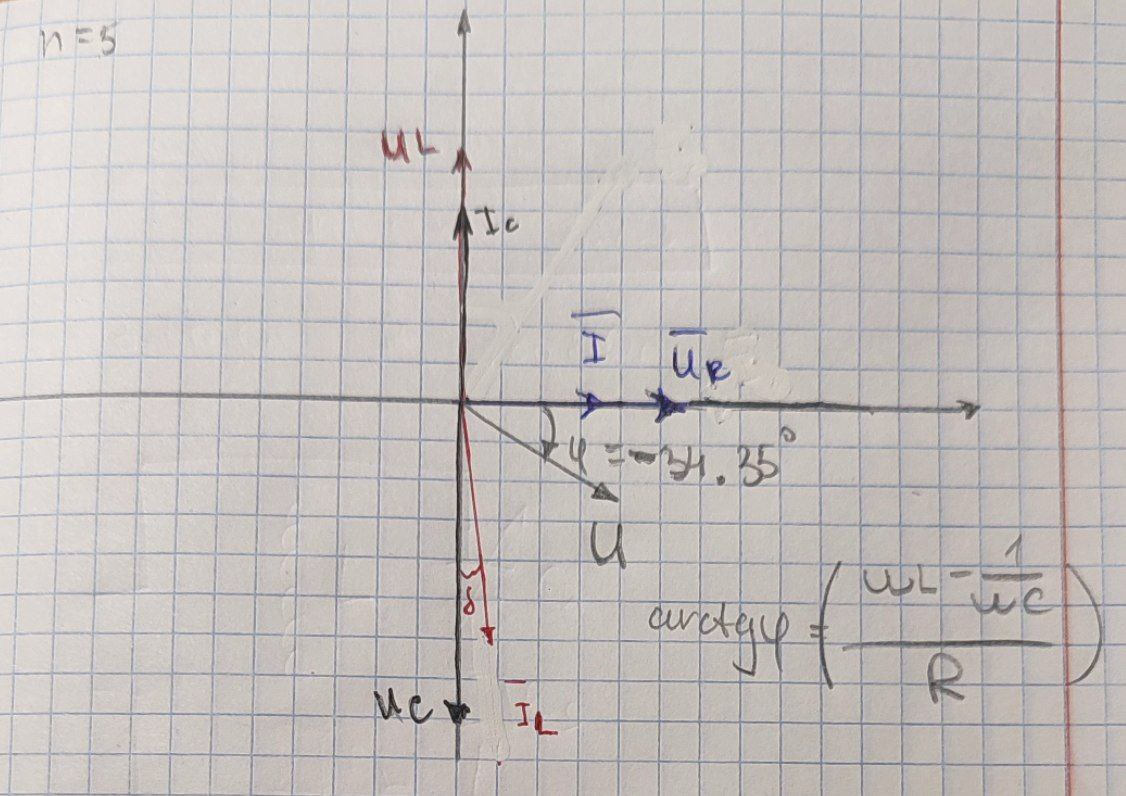
\includegraphics[width = 0.8\paperwidth, height = 0.4\paperheight]{vectr_diagr.jpg}
\caption{\textbf{Векторная диаграмма при n = 5}}    
\end{center}


\end{document}